\chapter{はじめに}
\thispagestyle{myheadings}

% **DIOCOMO2019 ========================================================**
\section{研究背景}
コロナウイルスの流行によって巣ごもり需要が拡大し,Netflixや YouTube,ニコニコ動画といった動画共有サイトの利用が広がっている.
これらのサービスはテレビ番組とは異なり,ユーザの好きな時間に好きなコンテンツを選択して視聴できるため,自分の好みやライフスタイルに合わせて映像コンテンツを楽しめる.
動画共有サイトなどに投稿された映像コンテンツは,利用の手軽さからスマートフォンを通して視聴される場合が多いが,その利点と引き換えにコンテンツが本来持っている視聴体験が失われる場合がある.
例えば映画館で上映される映像コンテンツは,大きなスクリーンと高音質なオーディオシステムを用いて投影されるのを前提として制作されている.そのため,映画館以外で視聴した場合には本来の映像美や迫力が減少してしまう.
特に,3Dや4DXで上映される映像コンテンツは,物理的/性能的な問題から自宅でのPCでは視聴体験を再現するのは不可能である.

動画プラットフォームとして,ニコニコ動画,YouTube,Netflix,Amazon Prime Video,Huluなどがあり,多様なジャンルの動画を提供しており,好みに合わせたコンテンツを視聴するのが可能.
ニコニコ動画は,動画を視聴している際に任意の再生時間に対して,コメントの投稿ができる.特に,生配信されている動画では視聴者がコメントを書き込むと,
同時に視聴している他の視聴者にもリアルタイムに反映され動画上にそのコメントが流れる.これにより,同時に視聴しているユーザ同士で文字をベースとしたコミュニケーションが取れるため,盛り上がりの共有が可能となる.
実際にコメントが流れている例を図\ref{nikoniko}に示す.

\begin{figure}[H]
    \centering
    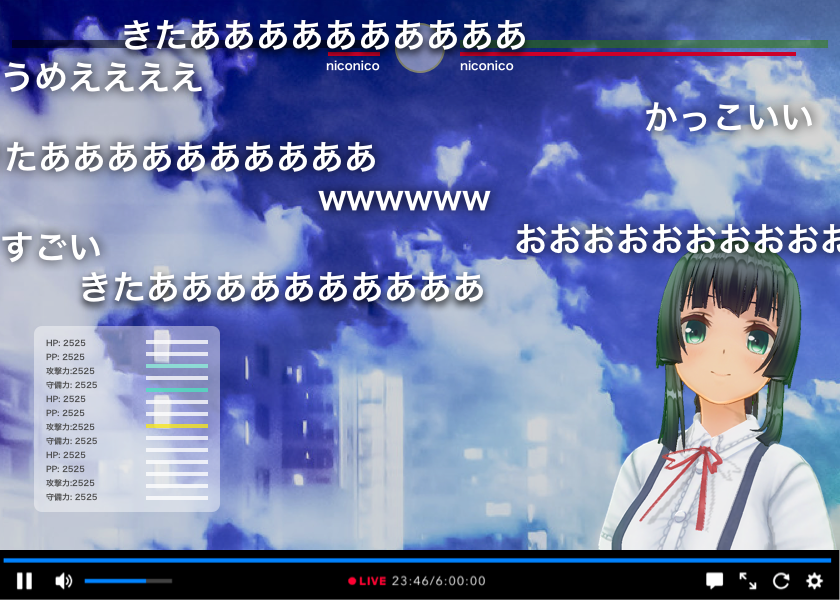
\includegraphics[width=10cm]{images/chapter1/nikoniko_grafu.png}
    \caption{視聴体験を向上させるサービス例 (ニコニコ動画の流れるコメント)}
    \label{nikoniko}
\end{figure}

YouTubeは,動画の中で最も視聴された部分を示すグラフがプログレスバー(再生バー)の上部に表示される(図\ref{youtube}).視聴数が多い箇所は高い山形となって表示され,ユーザーによって多く再生されたとわかる.
最も視聴数を集めた箇所のサムネイルには,「リプレイ回数が最も多い部分」と表示されるので視認性も高める効果がある.グラフは常時表示されるわけではなく,プログレスバーの赤いポインタで動画をスキップしているときに表示される.
グラフ機能の導入により,ユーザーは長尺の動画でもグラフを見れば「重要なポイント」と「見た方が良い箇所」がひと目で把握できる.プログレスバーのグラフ表示は,Web版YouTubeとモバイルアプリ版YouTubeの両方に提供されている.
再生画面上だけで操作・確認ができるので、コメント欄を確認する手間も省ける.

\begin{figure}[H]
    \centering
    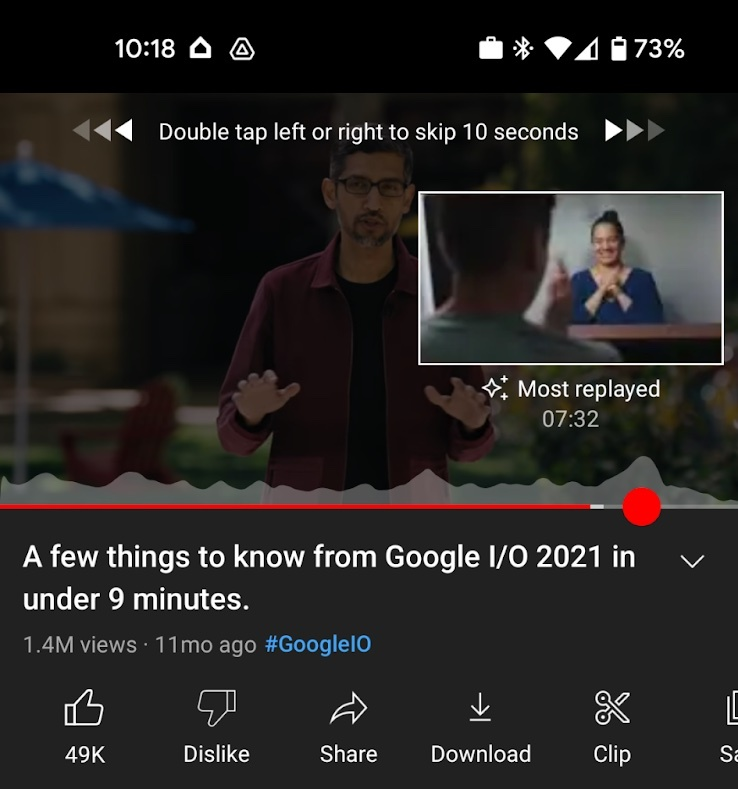
\includegraphics[width=10cm]{images/chapter1/YouTube.jpeg}
    \caption{視聴体験を向上させるサービス例 (Youtubeの最も視聴された部分を示すグラフ)}
    \label{youtube}
\end{figure}

人間の視野には中心視野と周辺視野と呼ばれる部分が存在する.中心視は視線を合わせた物をはっきりと認識する能力,周辺視は物をぼんやりとしか知覚できない代わりに全体像を瞬間的に知覚する能力である.ここで,周辺視は中心と比べて,
一度に得られる情報が多く,目に入った情報の処理も無意識的に行われるので目の疲労が少ないなどの利点がある.また,ホラー映画などのコンテンツは周辺視を利用してより視聴者の恐怖を高めるなどの手法をとっている.効率的に使用し動画の面白さを増幅できると考えられる.

技術的背景として,ニコニコ動画のコメントをリアルタイムに表示するためには,ネットワーク技術,通信プロトコル,動画配信技術の進歩が必要である.
LTE(ロングタームエボリューション)などの高速ネットワークの展開と, スマートフォンや様々なクラウドサービスの普及によりインターネットを流れるデータ量は急激に増大し,スマートフォンやパソコンを用いて,
日常的に様々なインターネットサービスが利用できるようになっている.新たなスマートデバイスやIoT(Internet of Things)サービスの普及,5G(第五世代移動通信システム)の商用展開などに伴い,暮らしを支えていく上で,インターネットへの接続はますます欠かせないものとなっている.
そして,インターネットにおいて広く利用されているのがTCP/IP(Transmission Control Protocol/Internet Protocol)と呼ばれるプロトコルである.
TCP/IPが普及した要因の一つとして,ネットワークの機能を必要最小限に低減するというコンセプトが挙げられる.ネットワークを高機能化すると一般的にコストが高くなる, 相互接続が難しくなる, 構築や保守が困難になる, といった弊害が発生する.
そのような問題を避け, シンプルなネットワークを指向するのがTCP/IPの特徴であると言える.
動画配信技術の進歩は大容量の動画データをストリーミングできる環境,高速なブロードバンド環境が整備され,ストリーミング配信の定額制サービスが急速に普及している.
ストリーミングとは,インターネットを介した動画配信や音楽配信に用いられる配信方式で、「オンデマンド型」と「ライブ型」の2種類がある。データのダウンロード後に視聴を開始するのではなく,データを受信しながら同時に随時再生していくという点がストリーミング方式の特徴である.
動画配信サービスを使ったストリーミング配信であれば,さまざまなデバイスに柔軟に対応できると同時にファイルが端末に残らない.

% **DIOCOMO2020 (ryoga)====================================================**
\section{目的とアプローチ}
本研究は,自宅での動画視聴に対する迫力の付加と,既存の映像コンテツの視聴体験を向上させるシステムを開発するを目的とする.
既存のコンテンツは,気軽に自宅や外出時のスマートフォンで,コンテンツを視聴できるようになっている.しかし,現在のコンテンツでは迫力のある映像体験を得るのは難しいといえる.
問題を解決するために,コンテンツに対してさらなる楽しみ方を提供する.具体的なアプローチとして,コンテンツを視聴しているときの生体データを使用し,盛り上がりがあるシーンに迫力を加える.つまりコンテンツ視聴時の生体データを集め,取得したデータを基に迫力を加える.
生体データを使用とは,そのコンテンツにおける盛り上がり部分を探し出すために,コンテンツ視聴時に取得した生体データを感情の判定に活用するのを意味する.
盛り上がりがあるシーンに迫力を加えるとは,盛り上がりの部分が抜き出された情報を使いコンテンツに効果を加える処理を意味する.
本研究では効果を加える具体的な方法として,より興奮した/より緊迫したという印象を与えるために,視聴している動画に対してエフェクトを画面全体に重畳表示する.

\section{論文構成}
本稿の構成は以下の通りである.2章では本研究に関連する研究として,生体データを用いた研究と重畳提示に関する研究を紹介する.
3章ではコンテンツ視聴時に生体データを取得し,コンテンツへ重畳提示する手法についての提案を行う.
第4章では評価実験を行い、本稿で提案した手法について生体データと重畳提示の二つに分けて評価する.5章ではまとめと今後の課題を述べる.

